\chapter{Electric control of skyrmion motion}
Since it was shown theoretically by Berger \cite{Berger1978,Berger1984,Berger1992,Berger1996} and Slonczewski \cite{Slonczewski1996} that a spin-polarized current could exert a torque on the magnetization in magnetic materials, there has been a lot of focus on electrical control of magnetization dynamics. Through the spin-transfer torque mechanism, one was able to switch the magnetization direction in a magnetic layer solely by applying a current through the material \cite{Myers1999,Sun1999,Katine2000}. This magnetization switching could for example be achieved by a current induced motion of magnetic domain walls \cite{Yamanouchi2004,Yamaguchi2004,Saitoh2004,Yamanouchi2006}. 

It has been shown that skyrmions can also be moved by applying a current, and they can be moved by a much weaker current than magnetic domain walls \cite{Jonietz2010,Yu2012}, which is the reason for the new interest in them. Recently it has also been shown that the motion of skyrmions can also be guided through the means of electric fields \cite{Upadhyaya2015}. It has also been discovered that through the help of constricted geometries and electrical currents, we can create skyrmions in chiral magnets \cite{Iwasaki2013,Sampaio2013,Jiang2015}. In addition we are able to detect skyrmions with an unpolarized current \cite{Monchesky2015}. These new developments will greatly help us in utilizing magnetic skyrmions in memory applications, such as racetracks. 

The goal of this chapter is to study the equations of motion for the skyrmion, both analytically and numerically, so that we can see how we can steer the motion of the skyrmion in the direction we want. We will consider the motion due to an electric field and an electric current, which will cause the magnetization to experience Rashba fields due to the broken inversion symmetry. An understanding of how we can control the motion of skyrmions by electrical means will be very useful in regards to how we can utilize skyrmions in memory applications.
\section{Skyrmion velocity}
The extended LLG equation that includes Rashba spin-orbit coupling and spin-transfer torques is given by
\begin{align}
\nonumber \frac{\partial \mathbold{M}}{\partial t} &= -\gamma'\mathbold{M}\times(\mathbold{H}_{\text{eff}}+\mathbold{H}_R-\frac{\beta}{M_s} \mathbold{M}\times\mathbold{H}_R) \\
&\hspace{4.5mm}+\frac{\alpha}{M_s}\mathbold{M}\times\frac{\partial\mathbold{M}}{\partial t} + b_J (\mathbold{\hat{j}}_e\cdot\mathbold{\nabla})\mathbold{M} - \frac{\beta b_J}{M_s} \mathbold{M}\times(\mathbold{\hat{j}}_e\cdot\mathbold{\nabla})\mathbold{M}, 
\label{eq:LLG_EC}
\end{align}
with the Rashba field $\mathbold{H}_R$ being given by
\begin{align}
\mathbold{H}_R = \frac{\alpha_R m_e}{\hbar \mu_0\mu_B}b_J (\mathbold{\hat{z}}\times\mathbold{\hat{j}}_e) = C_R b_J (\mathbold{\hat{z}}\times\mathbold{\hat{j}}_e)
\end{align}
and $b_J$ being a characteristic velocity
\begin{align}
    b_J = \frac{1}{1+\beta^2}\frac{\mu_B P j}{e M_s}.
\end{align}
This result was derived by Kim et al. in \cite{Kim2012} in a manner similar to the approach in Section \ref{sec:GeneralSTT}, where the Rashba Hamiltonian \eqref{eq:RashbaH} was included in the derivation with the s-d Hamiltonian. We now want to find this equation in the Thiele formalism, as it then goes from being a partial differential equation to being an algebraic equation in the velocity components. The terms involving the Rashba field $\mathbold{H}_R$ act as a magnetic field in the LLG equation, and we can therefore use the definition of the force from a magnetic field that is not aligned with the effective field in the Thiele equation as given by \eqref{eq:ThieleF}:
\begin{align}
\mathbold{F}_R &= -\mu_0\int \d V\sum_k (\mathbold{\nabla}M_k)\left[\mathbold{H}_R - \frac{\beta}{M_s}\mathbold{M}\times\mathbold{H}_R\right]_k.
\end{align}
This expression is calculated in Appendix \ref{app:F_RashbaThiele} and is found to be
\begin{align}
\mathbold{F}_R = -\mu_0 \pi\beta C_R b_J M_s d \int_0^{\infty} \d r \left(\frac{\partial \theta}{\partial r} r + \sin\theta\cos\theta \right) \mathbold{\hat{x}}
\end{align}
for a hedgehog skyrmion with $\psi = 0$ and $\theta(r=0)=\pi, \theta(r=\infty)=0$. We have assumed that the direction of the current is $\mathbold{\hat{j}}_e = \mathbold{\hat{x}}$. We will only consider these choices for the remainder of this chapter. This is reasonable, as for our particular choice of geometry with thin films (which is necessary to get a significant contribution from the electric field control) hedgehog skyrmions have the lowest energy due to interfacial DMI. We are also free to define the direction along the current to be the $x$-direction.

We now have the force resulting from Rashba spin-orbit coupling, the next step is then to find the force from an inhomogenous electric field. If we consider an electric field with a constant gradient, the field can then be written in cartesian and skyrmion coordinates as
\begin{subequations}
\begin{align}
E(\mathbold{r}) &= E_x x + E_y y \\
&= E_x x_0 + E_y y_0 + E_x r \cos\phi + E_y r \sin\phi,
\end{align}
\end{subequations}
with $\left( x_0,y_0\right)$ indicating the location of the skyrmion core. If we integrate this energy density over the entire film, we then find that the total energy contribution from the electric field becomes
\begin{align}
\nonumber U_{EF} &= \int \d V \epsilon_{EF} \\
\nonumber &= \eta \int_0^d \d z \int_0^{2\pi}\d \phi \int_0^{\infty}\d r\left( E_x x_0 + E_y y_0 + E_x r \cos\phi + E_y r \sin\phi \right) r \sin^2\theta \\
&= 2\pi\eta d\left(E_x x_0 + E_y y_0\right)\int_0^{\infty}\d r r \sin^2\theta.
\end{align}
Remembering that a gradient of the free micromagnetic energy will result in a force in the Thiele equation, as described by \eqref{eq:ThieleF}, we can write the force resulting from the inhomogenous electric field as
\begin{align}
\nonumber\mathbold{F}_E &= -\mathbold{\nabla}U_{EF} \\
&= -2\pi \eta d \left(E_x \mathbold{\hat{x}} + E_y \mathbold{\hat{y}}\right) \int_0^{\infty}\d r r \sin^2\theta.
\end{align}
The final equation in the Thiele formalism for our model can then be written as
\begin{align}
\mathbold{F}_R+\mathbold{F}_E + \mathbold{G} \times\left(\mathbold{v}+b_J\mathbold{\hat{j}}_e\right) + D\left(\alpha\mathbold{v}+\beta b_J \mathbold{\hat{j}}_e\right) = 0,
\end{align}
where we remember the definitions of the gyrovector $\mathbold{G}$ and dissipation factor $D$ to be
\begin{subequations}
\begin{align}
\mathbold{G} &= \frac{2\pi M_s\mu_0 d}{\gamma'}\left[\cos\theta\right]_{\theta(r=0)}^{\theta(r=\infty)} \mathbold{\hat{z}}\\
D &= - \frac{\pi M_s \mu_0 d}{\gamma '} \int_0^{\infty} \d r \left(r\left(\frac{\partial \theta}{\partial r}\right)^2+\frac{\sin^2\theta}{r}\right).
\end{align}
\end{subequations}
If we divide this equation by the length of $\mathbold{G}$, the non-trivial equations we end up with are
\begin{subequations}
\label{eq:EquationsMotionElectricControl}
\begin{align}
- R b_J - C_E E_x - \dot{y}_0 - \alpha_C \dot{x}_0 - \beta_C b_J &= 0, \\
-C_E E_y + \dot{x}_0 + b_J -\alpha_C\dot{y}_0 &= 0,
\end{align}
\end{subequations}
where we have made the following definitions:
\begin{subequations}
\begin{align}
\alpha_C &= \frac{\alpha}{4} \int_0^{\infty} \d r \left(r\left(\frac{\partial \theta}{\partial r}\right)^2+\frac{\sin^2\theta}{r}\right), \\
\beta_C &=\frac{\beta}{4} \int_0^{\infty} \d r \left(r\left(\frac{\partial \theta}{\partial r}\right)^2+\frac{\sin^2\theta}{r}\right), \\
R &= \frac{\gamma'\beta C_R}{4} \int_0^{\infty} \d r \left(\frac{\partial \theta}{\partial r} r + \sin\theta\cos\theta \right), \label{eq:Rconst}\\
C_E &= \frac{\gamma' \eta}{2\mu_0 M_s}\int_0^{\infty}\d r r\sin^2\theta.
\end{align}
\end{subequations}
Solving the equations in \eqref{eq:EquationsMotionElectricControl} for $\dot{x}_0$ and $\dot{y}_0$ one finally ends up with the velocity components of the motion of a skyrmion under the influence of spin-transfer torque, Rashba spin-orbit coupling and an inhomogenous electric field:
\begin{subequations}
\label{eq:ElectricalSkyrmionVComponents}
\begin{align}
\dot{x}_0 &= - \frac{1+\alpha_C(\beta_C + R)}{\alpha_C^2+1}b_J + \frac{C_E}{\alpha_C^2+1}E_y - \frac{\alpha_C C_E}{\alpha_C^2+1}E_x, \\
\dot{y}_0 &= \frac{\alpha_C-(\beta_C + R)}{\alpha_C^2+1}b_J - \frac{C_E}{\alpha_C^2+1}E_x - \frac{\alpha_C C_E}{\alpha_C^2+1}E_y.
\end{align}
\end{subequations}
From this result we can see the effects of RSOC and an electric field gradient on the velocity of the skyrmion center of mass. The RSOC has the same impact on the motion as the non-adiabatic STT, and appears as a correction to $\beta_C$ in the equations of motion. Note that only the term proportional to $\beta\mathbold{M}\times\mathbold{H}_R$ has an impact on the skyrmion dynamics, as a constant magnetic field like $\mathbold{H}$ can not induce a rigid motion of the skyrmion because there is no energy gain for it to move elsewhere. The constant field $\mathbold{H}_R$ can, however, induce a deformation of the skyrmion. For example, a constant external magnetic field pointing along the $z$-direction perpendicular to the skyrmion plane has an effect on the skyrmion size, much like magnetic anisotropy. If this external field is alternating, the field can cause the skyrmion size to shrink and increase periodically \cite{Mochizuki2012}, and in nanodots it can even be used to switch the magnetization of the core \cite{Zhang2015}. In our case the magnetic field experienced due to the Rashba effect lies in the skyrmion plane, and one would therefore expect it to have other deformation modes than a field pointing perpendicular to the skyrmion plane. To understand the effect of the non-uniform Rashba field proportional to $\beta\mathbold{M}\times\mathbold{H}_R$ we can compare it to the adiabatic STT in \eqref{eq:STT_Adiabatic_Macro}. The term in the LLG equation can be written as $\gamma\beta\mathbold{M}\times(\mathbold{M}\times\mathbold{H}_R)/M_s = -(\gamma\beta C_R b_J/M_s)\mathbold{M}\times(\mathbold{\hat{H}}_R\times\mathbold{M})$. This is very similar to the adiabatic STT acting on a magnetization $\mathbold{M}_j$ from a current that was polarized by passing through a magnetization $\mathbold{M}_i$. This torque was proportional to $-\mathbold{M}_j\times(\mathbold{M}_i\times\mathbold{M}_j)$. With the exception of the different torque magnitudes, the only difference is that the polarizing magnetic layer $\mathbold{M}_i$ is replaced by the Rashba field $\mathbold{H}_R$. This torque then originates from the conduction electrons that are polarized in the direction of the Rashba field. The direction of this field is given by $\mathbold{\hat{H}}_R=\mathbold{\hat{z}}\times\mathbold{\hat{j}}_e$. When the current is passing in the $x$-direction as we have considered so far, this field points in the $y$-direction. As this is generates a component of the spin polarization of the current that can be perpendicular to the local magnetization, it would explain why the torque behaves as the non-adiabatic STT. We now compare the driving torque resulting from RSOC more closely to the non-adiabatic STT. The driving torque from RSOC can be written as
\begin{align}
    \nonumber \gamma\beta\mathbold{m}\times\left(\mathbold{M}\times\mathbold{H}_R\right) &= \gamma\beta M_s\left(\left(\mathbold{m}\cdot\mathbold{H}_R\right)\mathbold{m}-\mathbold{H}_R\right) \\
    &=     
    \gamma\beta M_s C_R b_J
    \begin{pmatrix}
     \sin^2\theta\sin\Phi\cos\Phi \\
     \sin^2\theta\sin^2\Phi-1 \\
     \sin\theta\cos\theta\sin\Phi
    \end{pmatrix},
\end{align}
while the non-adiabatic STT can be written as 
\begin{align}
    -\beta b_J\mathbold{m}\times\left(\mathbold{\hat{j}}_e\cdot\mathbold{\nabla}\right)\mathbold{M} =     
    -\beta b_J M_s
    \begin{pmatrix}
     -\sin\Phi\cos\phi\partial_r\theta + \sin\theta\cos\theta\cos\Phi\sin\phi/r \\
     \cos\Phi\cos\phi\partial_r\theta + \sin\theta\cos\theta\sin\Phi\sin\phi/r \\
     -\sin^2\theta\sin\phi/r
    \end{pmatrix},
\end{align}
where we have used that $\partial_x\theta = -\sin\phi/r\partial_r\theta$ and $\partial_x\Phi = -\sin\phi/r$. If we integrate over the skyrmion plane, the only non-vanishing components in both torques in the $\psi=0$ case ($\Phi=\phi$) is the $y$-component. In addition, we see by performing this integration that we get the integral appearing in the RSOC term in \eqref{eq:Rconst}.

The electric field gradient introduces new terms to the velocity of the skyrmion. We can see that the skyrmion tends to move in a direction perpendicular to the electric field gradient, along $\mathbold{\hat{z}}\times(-\nabla E)$. In addition to the motion perpendicular to the gradient, the Gilbert damping also causes a damped motion in the opposite direction of the field gradient, moving the skyrmion to a lower energy state. The damped motion is relatively easy to understand, as it is nothing else than a relaxation of the magnetization to a lower energy. The motion of the skyrmion along the equipotential lines is a bit less intuitive, however. The reason for this motion is the Magnus force, resulting from the topology of the skyrmion. Initially the skyrmion experiences a force against the electric field gradient. At this point this is the only force acting on the skyrmion, as the Magnus force is only existent when the skyrmion moves. The skyrmion therefore drifts down to a lower energy state to begin with. However, as the the skyrmion starts to move the Magnus force kicks in, as the motion of the skyrmion induces an emergent electric field perpendicular to its motion, as described in Section \ref{sec:Berry}. This new force changes the direction of the skyrmion motion, until the motion is such that the Magnus force and the force from the inhomogeneous energy landscape cancel out, as illustrated in Figure \ref{fig:SkyrmionPotentialLineMotion}. The resulting motion is a Hall-like motion along the equipotential lines. This behaviour that we see from the electric field is analogous to the motion a skyrmion would have in the presence of an electric field in multiferroic insulators \cite{Liu2013}. The mechanism behind the motion due to the electric field is different, however. In multiferroic insulators the electric field couples to the dipole moment of the skyrmion, while in this ferromagnetic metal the motion is caused by a shift in the energy landscape due to the modification of the anisotropic energy by the voltage induced magnetic anisotropy. 

\begin{figure}[h!]
\centering
  \centering
  \begin{tikzpicture}
\node[above right] (img) at (0,0) {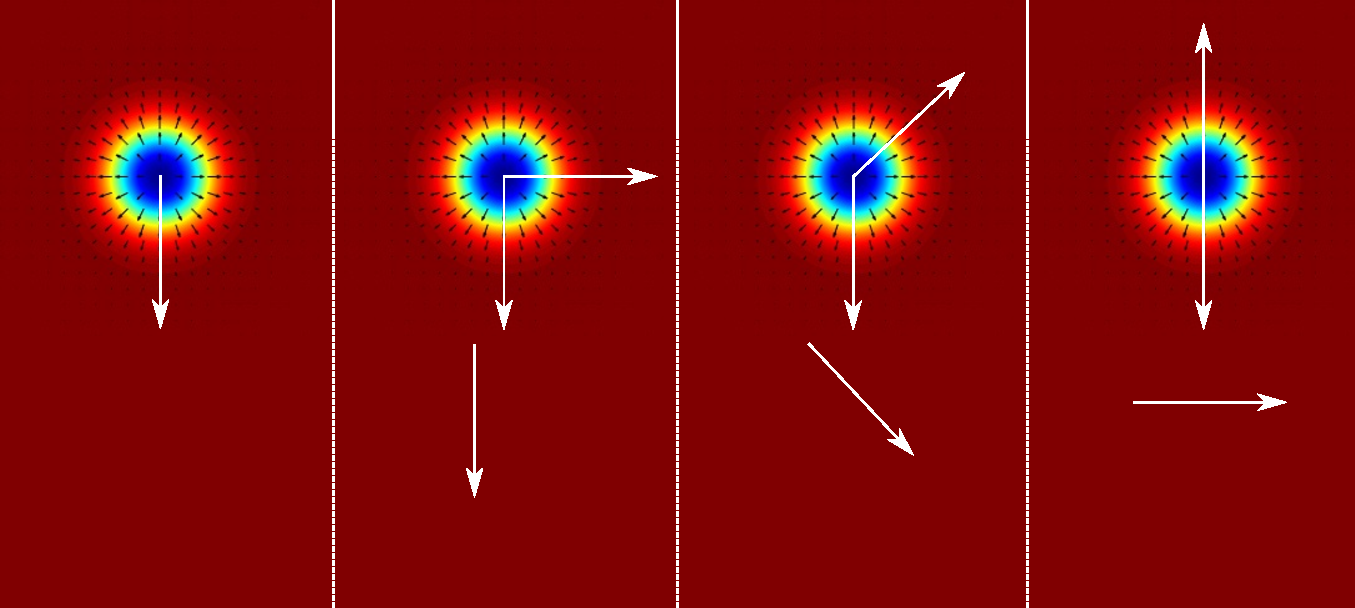
\includegraphics[width=1\textwidth]{Figures/SkyrmionPotentialLineMotionv2}};
\node at (60pt,15pt) {\textcolor{white}{\Large{$t = t_0$}}};
\node at (177pt,15pt) {\textcolor{white}{\Large{$t = t_1$}}};
\node at (294pt,15pt) {\textcolor{white}{\Large{$t = t_2$}}};
\node at (411pt,15pt) {\textcolor{white}{\Large{$t = t_3$}}};
\node at (40pt,120pt) {\textcolor{white}{\Large{$\mathbold{F}_E$}}};
\node at (155pt,120pt) {\textcolor{white}{\Large{$\mathbold{F}_E$}}};
\node at (270pt,120pt) {\textcolor{white}{\Large{$\mathbold{F}_E$}}};
\node at (385pt,120pt) {\textcolor{white}{\Large{$\mathbold{F}_E$}}};
\node at (60pt,60pt) {\textcolor{white}{\Large{$\mathbold{v}=0$}}};
\node at (175pt,60pt) {\textcolor{white}{\Large{$\mathbold{v}$}}};
\node at (290pt,60pt) {\textcolor{white}{\Large{$\mathbold{v}$}}};
\node at (405pt,60pt) {\textcolor{white}{\Large{$\mathbold{v}$}}};
\node at (200pt,180pt) {\textcolor{white}{\Large{$\mathbold{G}\times\mathbold{v}$}}};
\node at (290pt,180pt) {\textcolor{white}{\Large{$\mathbold{G}\times\mathbold{v}$}}};
\node at (380pt,180pt) {\textcolor{white}{\Large{$\mathbold{G}\times\mathbold{v}$}}};
\end{tikzpicture}
\caption{The initial motion due to the force from the spatially varying electric field is redirected due to the appearance of the Magnus force when the skyrmion starts to move. In equilibrium we have a Hall-like motion along the equipotential lines in the absence of Gilbert damping.}
\label{fig:SkyrmionPotentialLineMotion}
\end{figure}

\section{Numerical integrals}
The solution of the skyrmion velocity depends on parameters that are functions of three different integrals. These integrals depend on the solution of $\theta(r)$ that is obtained numerically by solving \eqref{eq:ODEtheta}. As our solution of $\theta$ is a numerical function, the integrals have to be calculated numerically as well. In \eqref{eq:ODEtheta} the only variable parameter is the skyrmion parameter $C = AK/D^2$, so the integrals can be expressed as functions of $C$ and for some of the integrals a dimensional scaling factor. The three integrals that we need to evaluate are
\begin{subequations}
\begin{align}
I_1 &= \int_0^{\infty} \textrm{d} \tilde{r} \left(\tilde{r}\left(\frac{\partial \theta}{\partial \tilde{r}}\right)^2+\frac{\sin^2\theta}{\tilde{r}}\right), \\
I_2 &= \frac{A}{D} \int_0^{\infty} \textrm{d} \tilde{r} \left(\frac{\partial \theta}{\partial \tilde{r}} \tilde{r} + \sin\theta\cos\theta \right), \\
I_3 &= \frac{A^2}{D^2}\int_0^{\infty} \textrm{d} \tilde{r} \tilde{r}\sin^2\theta.
\end{align}
\end{subequations}
Here the solution of $\theta$ inside the integrals is given in the dimensionless length scale $\tilde{r} = r\cdot D/A$. The resulting integrals as functions of $C$ are shown in Figure \ref{fig:ThetaInts}.
\begin{figure}[h!]
\centering
\begin{subfigure}{.49\textwidth}
  \centering
  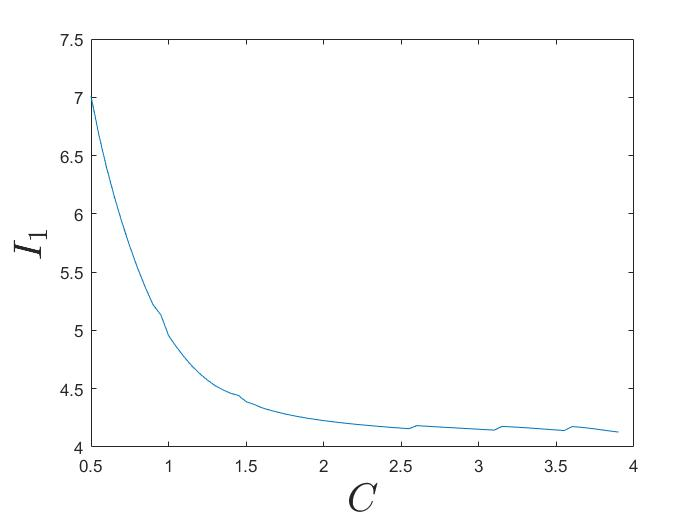
\includegraphics[width=\linewidth]{Figures/I1Plot.jpg}
  \caption{}
  \label{fig:ThetaInt1}
\end{subfigure}
\begin{subfigure}{.49\textwidth}
  \centering
  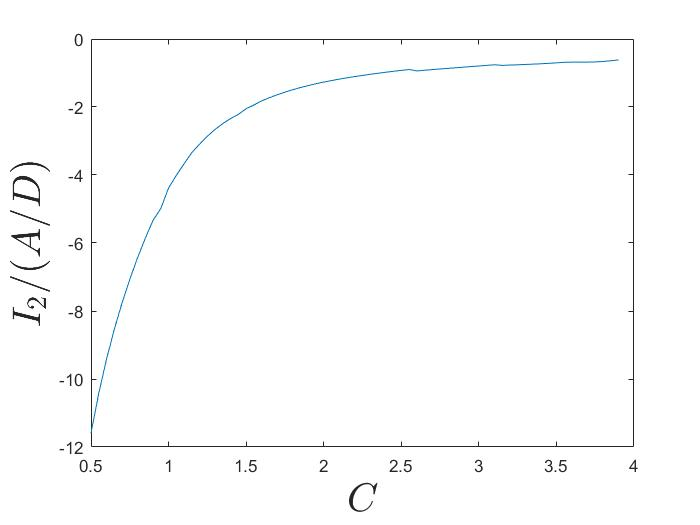
\includegraphics[width=\linewidth]{Figures/I2Plot.jpg}
  \caption{}
  \label{fig:ThetaInt2}
\end{subfigure}
\linebreak
\begin{subfigure}{.49\textwidth}
  \centering
  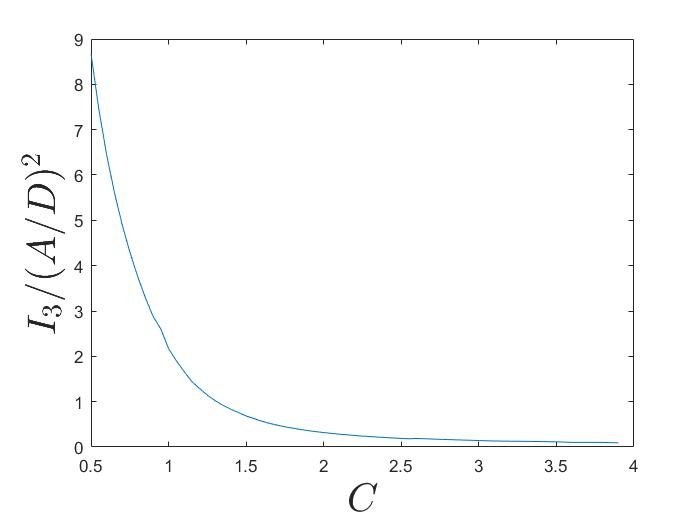
\includegraphics[width=\linewidth]{Figures/I3Plot.jpg}
  \caption{}
  \label{fig:ThetaInt3}
\end{subfigure}
\caption{Numerical evaluations of the integrals \textbf{(a)} $I_1$, \textbf{(b)} $I_2$ and \textbf{(c)} $I_3$ as a function of the skyrmion parameter $C$.}
\label{fig:ThetaInts}
\end{figure}

\section{Pinning, threshold currents and field gradients}
As with domain walls, there is also a threshold current or field that is necessary for skyrmions to start moving, even though our previous results do not reflect this. In the case of skyrmions this threshold current is much weaker than the case of domain walls \cite{Jonietz2010}. The reason for this reluctance to move is pinning centers, which have much less impact on the motion of skyrmions than that of domain walls, but have an impact nonetheless. To model the effect of pinning centers on skyrmion motions at low current densities or weak electric fields, one can introduce a pinning force in the Thiele equation \eqref{eq:Thiele}. The equation of interest then becomes
\begin{align}
\label{eq:PinningThiele}
\mathbold{F}_{\textrm{pin}}+\mathbold{F}_R+\mathbold{F}_E + \mathbold{G} \times\left(\mathbold{v}+b_J\mathbold{\hat{j}}_e\right) + D\left(\alpha\mathbold{v}+\beta b_J \mathbold{\hat{j}}_e\right) = 0.
\end{align}
The phenemenological pinning force $\mathbold{F}_{\textrm{pin}}$ is usually written as \cite{Everschor2012, IwasakiNagaosa2013}.
\begin{align}
\mathbold{F}_{\textrm{pin}} = -4\pi v_{\textrm{pin}} f(\frac{v}{v_{\textrm{pin}}}) \frac{\mathbold{v}}{v},
\end{align}
where the function $f(\frac{v}{v_{\textrm{pin}}})$ goes towards unity for small skyrmion velocities $v$. This is to ensure that the force does not vanish as $v\rightarrow 0$, but there is a constant force barrier that the skyrmion needs to overcome to have a velocity greater than zero. In the low velocity limit one therefore approximates the pinning force by
\begin{align}
\mathbold{F}_{\textrm{pin}} = - v_{\textrm{pin}} \frac{\mathbold{v}}{v},
\end{align}
where the forces are normalized in a way so that the gyrovector $\mathbold{G} = (0, 0, 1)$. The non-trivial equations we then get from \eqref{eq:PinningThiele} are
\begin{subequations}
\label{eq:PinningThieleComponents}
\begin{align}
\label{eq:PinningThieleA}
-\dot{y}_0 - \beta_Cb_J - \alpha_C\dot{x}_0 - v_{\textrm{pin}}\frac{\dot{x}_0}{v} + F_x &= 0, \\
\label{eq:PinningThieleB}
b_J + \dot{x}_0 - \alpha_C\dot{y}_0 - v_{\textrm{pin}}\frac{\dot{y}_0}{v} + F_y &= 0,
\end{align}
\end{subequations}
where $F_x$ and $F_y$ are the $x-$ and $y-$ components of the total force $\mathbold{F}_R + \mathbold{F}_E$ resulting from Rashba spin-orbit coupling and voltage induced magnetic anisotropy respectively. In the case of $F_x = F_y = 0$, one can see that if one makes the substitution
\begin{align}
\alpha_C \rightarrow \alpha_C+\frac{v_{\textrm{pin}}}{v}
\end{align}
the equations of motion are exactly the same as for the case of the motion of a skyrmion due to a spin-polarized current. The solutions of $\dot{x}_0$ and $\dot{y}_0$ are known in this case, and one can therefore make the substitution of $\alpha_C$ above into these solutions to get the solutions in the presence of pinning:
\begin{subequations}
\begin{align}
\dot{x}_0 &= -\frac{1+(\alpha_C+\frac{v_{\textrm{pin}}}{v})\beta_C}{(\alpha_C+\frac{v_{\textrm{pin}}}{v})^2+1}b_J, \\
\dot{y}_0 &= \frac{(\alpha_C+\frac{v_{\textrm{pin}}}{v}) - \beta_C}{(\alpha_C+\frac{v_{\textrm{pin}}}{v})^2+1}b_J.
\end{align}
\end{subequations}
As one can see, these solutions depend on the total skyrmion velocity $v$. To determine this velocity we use the relation $v^2 = \dot{x}_0^2+\dot{y}_0^2$ and the solutions above, which gives us the equation
\begin{align}
v^2 = \frac{\beta_C^2+1}{(\alpha_C+\frac{v_{\textrm{pin}}}{v})^2+1}b_J^2.
\end{align}
Rearranging this equation one can get the following second order equation in $v$:
\begin{align}
(\alpha_C^2+1)v^2+(2\alpha_Cv_{\textrm{pin}})v + (v_{\textrm{pin}}^2-(\beta_C^2+1)b_J^2) = 0.
\end{align}
The solution to this equation is given by
\begin{align}
v = \frac{\sqrt{(\alpha_Cv_{\textrm{pin}})^2+(\alpha_C^2+1)\left[(\beta_C^2+1)b_J^2-v_{\textrm{pin}}^2\right]}-\alpha_Cv_{\textrm{pin}}}{\alpha_C^2+1},
\end{align}
where the positive solution has been chosen as that is the only solution that can give a positive $v$. This solution in $v$ differs from the solution given by Iwasaki et al. \cite{IwasakiNagaosa2013} by the term outside of the square root, but the solutions of $\dot{x}_0$ and $\dot{y}_0$ are in agreement. As our solution of $v$ is consistent with our solutions of $\dot{x}_0$ and $\dot{y}_0$, and if one plugs our solutions into the equations in \eqref{eq:PinningThieleComponents} they are satisfied in the case $F_x = F_y = 0$, it is concluded that our solutions are correct. 

So far we have only discussed pinning of the spin-polarized current driven skyrmion motion, but it is also of interest to find the same results in the presence of Rashba spin-orbit coupling and an imhomogenous electric field perpendicular to the film. In other words, we must solve \eqref{eq:PinningThieleComponents} when $F_x \neq 0$ and $F_y \neq 0$. We apply the same trick again where we try to incorporate $F_x$ and $F_y$ into similar variables in the equations we already have a solution for. $F_x$ and $F_y$ are both independent of $\dot{x}_0$, $\dot{y}_0$ and $v$, we must therefore try to include them in other terms also independent of these variables. In \eqref{eq:PinningThieleA} the only term independent of these is $-\beta_Cb_J$, and in \eqref{eq:PinningThieleB} the term is $b_J$. If we define new variables $\tilde{\beta}_C$ and $\tilde{b}_J$ that satisfy
\begin{subequations}
\begin{align}
-\tilde{\beta}_C\tilde{b}_J &= -\beta_Cb_J + F_x, \\
\tilde{b}_J &= b_J + F_y,
\end{align}
\end{subequations}
meaning they have the following definitions:
\begin{subequations}
\begin{align}
\tilde{\beta}_C &= \frac{\beta_Cb_J-F_x}{b_J+F_y}, \\
\tilde{b}_J &= b_J + F_y,
\end{align}
\end{subequations}
the equations have the same form as before with $\beta_C \rightarrow \tilde{\beta}_C$ and $b_J \rightarrow \tilde{b}_J$. The total force components resulting from $\mathbold{F}_R+\mathbold{F}_E$ are
\begin{subequations}
\begin{align}
F_x &= -C_E E_x - Rb_J, \\
F_y &= -C_E E_y.
\end{align}
\end{subequations}
If we plug these into $\tilde{\beta}_C$ and $\tilde{b}_J$ and make the substitutions in our previous solutions of $\dot{x}_0$, $\dot{y}_0$ and $v$ from the current driven case, we end up with the solutions
\begin{subequations}
\begin{align}
\dot{x}_0 &= -\frac{1+(\alpha_C+\frac{v_{\textrm{pin}}}{v})(\beta_C+R)}{(\alpha_C+\frac{v_{\textrm{pin}}}{v})^2+1}b_J + \frac{C_E}{(\alpha_C+\frac{v_{\textrm{pin}}}{v})^2+1}E_y - \frac{(\alpha_C+\frac{v_{\textrm{pin}}}{v})C_E}{(\alpha_C+\frac{v_{\textrm{pin}}}{v})^2+1}E_x, \\
\dot{y}_0 &= \frac{(\alpha_C+\frac{v_{\textrm{pin}}}{v})-\beta_C - R}{(\alpha_C+\frac{v_{\textrm{pin}}}{v})^2+1}b_J - \frac{C_E}{(\alpha_C+\frac{v_{\textrm{pin}}}{v})^2+1}E_x - \frac{(\alpha_C+\frac{v_{\textrm{pin}}}{v}) C_E}{(\alpha_C+\frac{v_{\textrm{pin}}}{v})^2+1}E_y, \\
\label{eq:PinningVElectrical}
v &= \frac{\sqrt{(\alpha_Cv_{\textrm{pin}})^2+(\alpha_C^2+1)\left[(\beta_Cb_J+Rb_J+
C_EE_x)^2+(b_J-C_EE_y)^2-v_{\textrm{pin}}^2\right]}-\alpha_Cv_{\textrm{pin}}}{\alpha_C^2+1}.
\end{align}
\end{subequations}
It can be seen that in the limit of no pinning ($v_{\textrm{pin}} \rightarrow 0$) the results for $\dot{x}_0$ and $\dot{y}_0$ are in agreement with \eqref{eq:ElectricalSkyrmionVComponents}. From the expression for $v$ in \eqref{eq:PinningVElectrical} it is also possible to determine the threshold current or electric field gradient necessary for the solution of $v$ to be greater than zero. If we first consider the case where the skyrmion motion is solely driven by a spin-polarized current, one finds that the skyrmion moves when $b_J > b_J^{\textrm{(crit)}}$ with
\begin{align}
b_J^{\textrm{(crit)}} = \frac{1}{1+\beta^2} \frac{\mu_BP}{eM_s}j_e^{\textrm{(crit)}}= \frac{v_{\textrm{pin}}}{\sqrt{(\beta_C+R)^2+1}}.
\end{align}
In the field driven case where the skyrmion motion is solely driven by an inhomogenous electric field applied perpendicular to the film, one finds that the skyrmion moves when the field gradient $E_g = \sqrt{E_x^2+E_y^2}$ is greater than some critical value
\begin{align}
E_g^{\textrm{(crit)}} = \frac{v_{\textrm{pin}}}{C_E}.
\end{align}
The numerical values of $b_J^{\text{(crit)}}$ and $E_g^{\text{(crit)}}$ for different values of the skyrmion parameter $C$ are shown in Figure \ref{fig:CritCurrentField}. As one can see, the behavior of the critical current and field gradient are quite different. The critical current is a strictly decreasing function of $C$, but the decrease is only significant for high values of $\beta$. The critical field gradient, however, is a strictly increasing function of $C$, and increases significantly from $C = 0.5$ to $C = 2.5$. If the unit length $A/D$ is kept constant, the size of the skyrmion decreases with increasing $C$ (which can be seen from Figure \ref{fig:ThetaProfile}). Still assuming that $A/D$ is kept constant, one sees that in the current driven case smaller skyrmions have a lower critical current, while in the electric field driven case larger skyrmions have a lower critical field gradient. This can be understood rather intuitively. The non-adiabatic spin-transfer torque acts as a drag force on the skyrmion in the Thiele equation. This drag force attempts to move the skyrmion in the direction of the conduction electrons. Normally the total non-adiabatic STT is larger for larger skyrmions, but with the presence of RSOC we get an effectively reduced non-adiabatic STT. This reduction is greater for larger skyrmions due to the larger area where the conduction electrons polarized along the Rashba field can transfer their spin to the local magnetization. Because of this effective reduction of the non-adiabatic STT larger skyrmions experience less drag along the motion of the conduction electrons, and smaller skyrmions then require a smaller current to be moved than large ones. If RSOC was not present the situation would be reversed, as there is no reduction of the drag resulting from non-adiabatic STT, and larger skyrmions would have a lower critical current due to the larger drag force acting on them. For the electric field driven case the spatial variation of the free energy has a larger impact on a large skyrmion than a small skyrmion.

\begin{figure}[h!]
\centering
\begin{subfigure}{.49\textwidth}
  \centering
  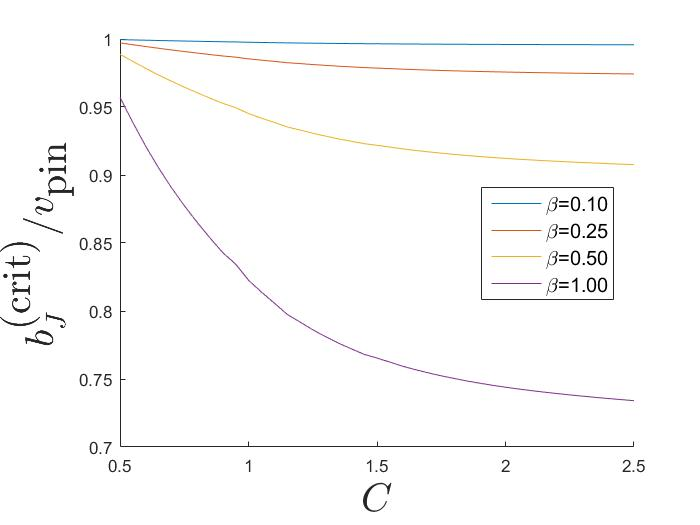
\includegraphics[width=\linewidth]{Figures/CritCurrent.jpg}
  \caption{}
  \label{fig:CritCurrent}
\end{subfigure}
\begin{subfigure}{.49\textwidth}
  \centering
  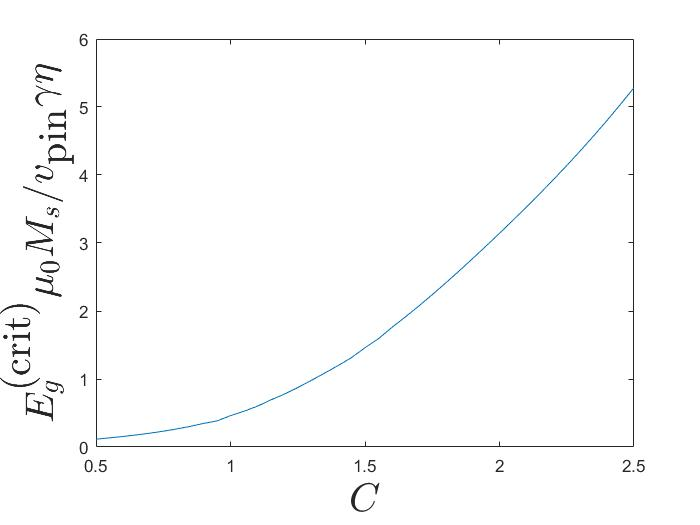
\includegraphics[width=\linewidth]{Figures/CritField.jpg}
  \caption{}
  \label{fig:CritField}
\end{subfigure}
\caption{\textbf{(a)} The critical current density and \textbf{(b)} the critical field gradient as a function of the skyrmion parameter $C$.}
\label{fig:CritCurrentField}
\end{figure}

\section{Numerical simulations}
In our analytical calculations in the previous sections we have solved the Thiele equation, which is a simplification of the LLG equation. The Thiele equation assumes that we have a rigid motion of the skyrmion, so that the motion of the skyrmion can be described by the motion of a key feature of the magnetization pattern such as the skyrmion core. Because of this, the Thiele equation can not describe whether the skyrmion becomes deformed during its motion or not. In some of the cases we have considered so far it is likely that there will at least be certain deformation of the skyrmion profile. The presence of RSOC and application of an electric field gradient to the system will cause the magnetization to experience magnetic fields that are not aligned with the effective field that stabilizes the skyrmion. To judge if our analytical results have any merit, we therefore solve the LLG equation numerically where we make no assumptions regarding the rigidness of the skyrmion motion. We can then compare our analytical results in the Thiele framework with the numerical results in the LLG framework to see if a rigid motion is a good approximation or not.
\subsection{The LLG equation as a parabolic equation}
The LLG equation is a partial differential equation that is first order in time, and contains first and second order spatial derivatives through the effective field from DMI and the exchange interaction in the skyrmion case. It should then be possible to write the LLG equation on the following form:
\begin{align}
\label{eq:LLG_PDE}
\bar{d}\mathbold{\dot{m}} - \nabla\cdot(\mathbold{\bar{c}}\otimes\nabla \mathbold{m}) + \bar{a}\mathbold{m} = \mathbold{f}.
\end{align}
Here $\mathbold{m}$ and $\mathbold{f}$ are vectors of length $N$, $\bar{d}$ and $\bar{a}$ are $N\times N$ matrices, and $\mathbold{\bar{c}}$ is a $N_{\textrm{dim}}\times N_{\textrm{dim}} \times N\times N$ tensor. For the case of the skyrmion, we have three magnetization components we need to solve for in a 2D plane, in other words $N = 3$ and $N_{\textrm{dim}}=2$. Equations on the form given by \eqref{eq:LLG_PDE} are solved by the \texttt{parabolic} function in \texttt{MATLAB}'s \texttt{PDE Toolbox}, which utilizes a finite element method. We then need to rewrite \eqref{eq:LLG_EC} to the form of \eqref{eq:LLG_PDE}. This was done and provided the following results:
\begin{subequations}
\begin{align}
\mathbold{f} &= 
 \begin{pmatrix}
  b_J\partial_x m_x - \beta b_J(m_y\partial_xm_z - m_z\partial_xm_y) + 2(m_y\partial_xm_x+m_y\partial_ym_y+m_z\partial_ym_z)\gamma D/(\mu_0M_s)\\
  b_J\partial_x m_y - \beta b_J(m_z\partial_xm_x-m_x\partial_xm_z)-2(m_z\partial_xm_z+m_x\partial_xm_x+m_x\partial_ym_y) \gamma D/(\mu_0M_s) -\beta H_R\\
  b_J\partial_xm_z - \beta b_J(m_x\partial_xm_y-m_y\partial_xm_x) - 2(m_x\partial_ym_z-m_y\partial_xm_z)\gamma D/(\mu_0M_s)
 \end{pmatrix}, \\
\bar{d} &= 
 \begin{pmatrix}
  1 & \alpha m_z & -\alpha m_y \\
  -\alpha m_z & 1 & \alpha m_x \\
  \alpha m_y & -\alpha m_x  & 1
 \end{pmatrix}, \\
 \bar{a} &= 
 \begin{pmatrix}
  -\gamma \beta H_R m_y & 2\gamma (K+\eta E) m_z/(\mu_0M_s) & -\gamma H_R \\
  -2\gamma (K+\eta E) m_z/(\mu_0M_s) & -\gamma\beta H_R m_y & 0 \\
  \gamma H_R & 0  & -\gamma \beta H_R m_y
 \end{pmatrix}, \\
  \mathbold{\bar{c}} &= 
 \begin{pmatrix}
  \bar{0} & 2\gamma Am_z\bar{I}/(\mu_0M_s) & -2\gamma Am_y\bar{I}/(\mu_0M_s) \\
  -2\gamma Am_z\bar{I}/(\mu_0M_s)  & \bar{0} & 2\gamma Am_x\bar{I}/(\mu_0M_s) \\
  2\gamma Am_y\bar{I}/(\mu_0M_s) & -2\gamma Am_x\bar{I}/(\mu_0M_s)  & \bar{0}
 \end{pmatrix},
\end{align}
\end{subequations}
with $\bar{0}$ being a $2\times 2$ matrix of zeros, and $\bar{I}$ the two-dimensional identity matrix. The $i$-th component of $\nabla\cdot(\mathbold{\bar{c}}\otimes\nabla \mathbold{m})$ is defined as
\begin{align}
    \left[\nabla\cdot(\mathbold{\bar{c}}\otimes\nabla \mathbold{m})\right]_i = \sum_{j=1}^{N}\left(\partial_xc_{i,j,1,1}\partial_x+\partial_xc_{i,j,1,2}\partial_y+\partial_yc_{i,j,2,1}\partial_x+\partial_yc_{i,j,2,2}\partial_y\right) m_j.
\end{align}
\subsection{Dimensional analysis}
When performing the numerical simulations it is necessary to do this using dimensionless quantities. We therefore need to define a unit length- and time-scale for the system based on our parameters. For the unit length-scale we continue to use the one defined in the numerical solution of the skyrmion profile in Section \ref{sec:Skyrmions}, which was $\tilde{r} = rD/A$. The unit length scale is therefore $\underline{r}=A/D$. For the time-scale of the system we choose one such that $\underline{t}\gamma K/\mu_0 M_s = 1$, in other words $\underline{t}=\mu_0 M_s/\gamma K$. We now use these definitions to find the scalings of the remaining parameters. The parameter $b_J$ is a velocity factor, and when its dimensionless counterpart is unity it takes on the value $\underline{r}/\underline{t} = \gamma A K/D\mu_0 M_s$. Moving on to the effective field terms from the DMI and exchange interaction, we need to consider spatial derivatives. These derivatives needs to be done in a dimensionless space. We can then see from the chain rule that $\partial_x = \underline{r}^{-1}\partial_{\tilde{x}}$. Each derivative will then carry with it a factor $D/A$ for the derivative to be done in dimensionless coordinates. We then note that the effective field originating from DMI has one spatial derivative, while the effective field originating from the exchange interaction has a double spatial derivative. As $A(D/A)^2 = D (D/A) = K/C$ these fields scale similarly in our dimensionless space. Since we have defined $\underline{t}\gamma K/\mu_0 M_s = 1$, we simply divide these effective fields by the factor $C = AK/D^2$ to get the right scaling. Lastly we consider the scaling of the Rashba field $H_R$. Due to the definition of the time-scale we must require that the dimensionless value of $\gamma H_R$ to be unity when $H_R = K/\mu_0 M_s$, which is the measure of field strength chosen in our simulations. A summary of the dimensional scalings is shown in Table \ref{tab:DimAnalysis}.
\begin{table}[h]
\begin{center}
  \caption{List of dimensionless quantities utilized in the numerical simulation and the scaling factor to get the correct unit and magnitude of the physical quantity.}
  \begin{tabular}{ c c c }
    \hline
    \text{Dimensionless quantity} & \text{Proper unit} & \text{Scaling factor} \\ \hline
    $t$ & s & $\mu_0M_s/\gamma K$ \\
    $r$ & m & $A/D$ \\
    $b_J$ & m/s & $\gamma K A/\mu_0 M_s D$ \\
    $H_R$ & A/m & $K/\mu_0 M_s$ \\
    $D\partial_{\tilde{x}}$ & J/m$^3$ & $D^2/A$ \\
    $A\partial_{\tilde{x}}^2$ &J/m$^3$ & $D^2/A$ \\
    \hline
  \end{tabular}
  \label{tab:DimAnalysis}
\end{center}
\end{table}

In Table \ref{tab:PhysicalConstants} we list some parameter values for a Ir|Co|Pt multilayer system \cite{Moreau-Luchaire2016} and 1 nm thick cobalt nanotracks \cite{ZhangEzawa2015}. The value of $\alpha_R$ is determined by using the values of $A$, $D$ and other physical constants in the relation \eqref{eq:DalphaR}. 
\begin{table}[h]
\begin{center}
  \caption{Table of physical quantities for a Ir|Co|Pt multilayer system and 1 nm thick cobalt nanotracks.}
  \begin{tabular}{ c c c c }
    \hline
    \text{Quantity} & \text{Unit} & \text{Ir|Co|Pt} & \text{Cobalt} \\ \hline
    $A$ & pJ/m & 10 & 15\\
    $D$ & mJ/m$^2$ & 1.75 & 4 \\
    $K$ & MJ/m$^3$ & 0.17 & 0.8 \\
    $M_s$ & MA/m & 0.96 & 0.58 \\
    $\alpha_R$ & peV$\cdot$m & 3.3 & 5.1 \\
    \hline
  \end{tabular}
  \label{tab:PhysicalConstants}
\end{center}
\end{table}

\subsection{Static case}
As a test case we will first simulate the LLG equation without any driving torques or fields as given by \eqref{eq:LLG}, where we give in the skyrmion profile solved numerically as an initial state. As the magnetization of the skyrmion is parallel with the effective field, which is why the skyrmion is a stable solution, we would expect the solution to be static ($\mathbold{M}(\mathbold{r},t) = \mathbold{M}(\mathbold{r},t=0)$).
\begin{figure}[h!]
\centering
\begin{subfigure}{.3\textwidth}
  \centering
  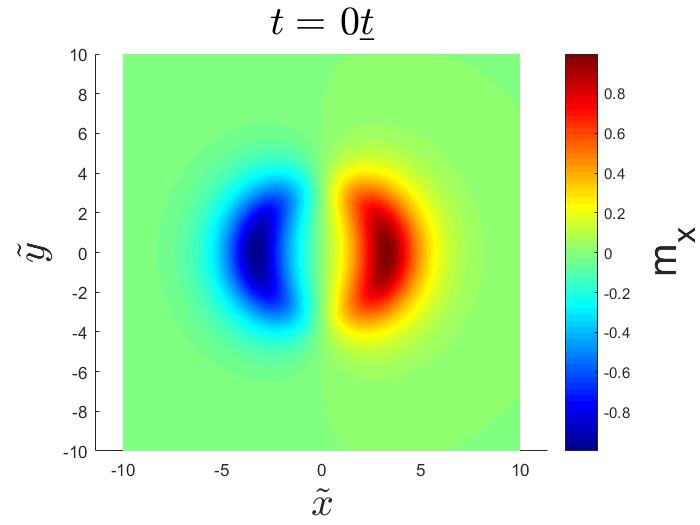
\includegraphics[width=\linewidth]{Figures/StaticSkyrmionMxT0.jpg}
  \caption{}
  \label{fig:StaticSkyrmionMxT0}
\end{subfigure}
\begin{subfigure}{.3\textwidth}
  \centering
  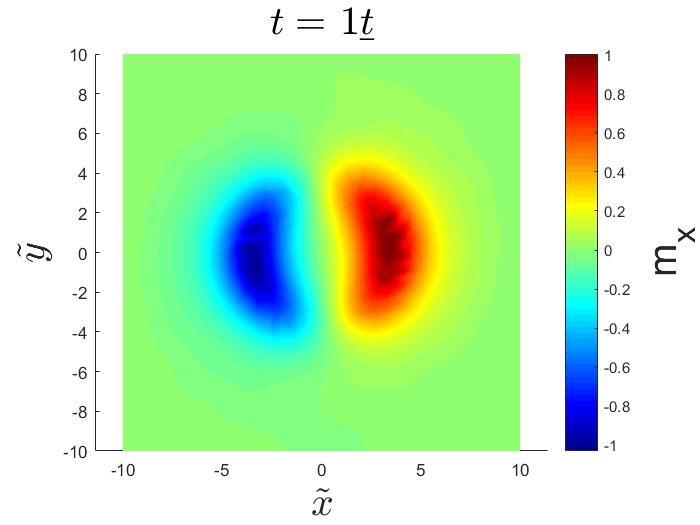
\includegraphics[width=\linewidth]{Figures/StaticSkyrmionMxT1.jpg}
  \caption{}
  \label{fig:StaticSkyrmionMxT1}
\end{subfigure}
\begin{subfigure}{.3\textwidth}
  \centering
  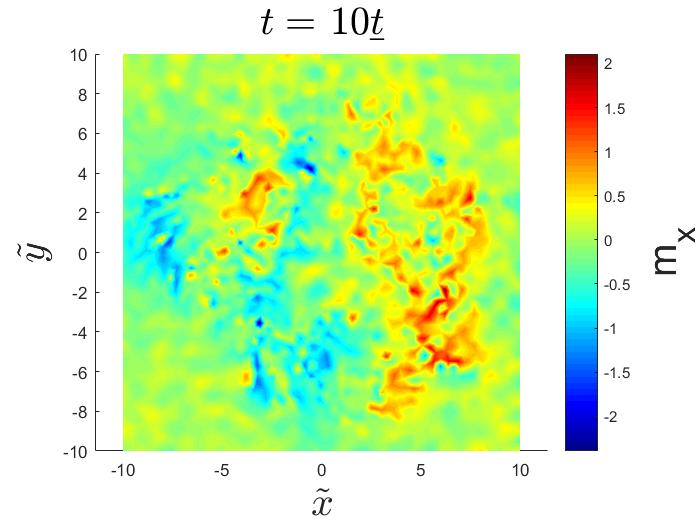
\includegraphics[width=\linewidth]{Figures/StaticSkyrmionMxT10.jpg}
  \caption{}
  \label{fig:StaticSkyrmionMxT10}
\end{subfigure}

\begin{subfigure}{.3\textwidth}
  \centering
  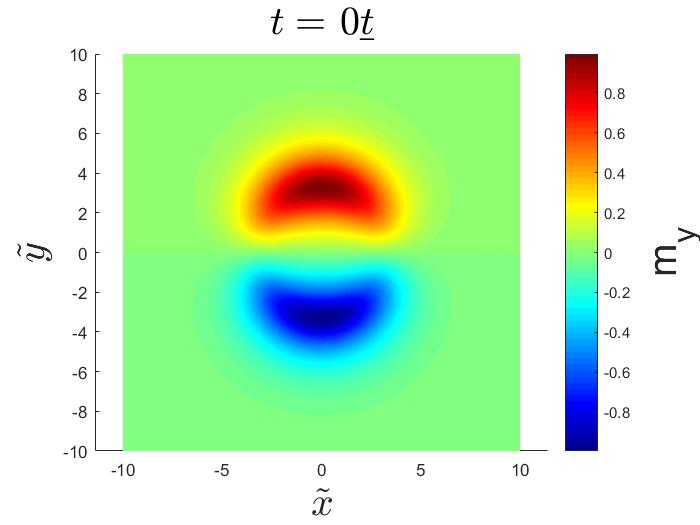
\includegraphics[width=\linewidth]{Figures/StaticSkyrmionMyT0.jpg}
  \caption{}
  \label{fig:StaticSkyrmionMyT0}
\end{subfigure}
\begin{subfigure}{.3\textwidth}
  \centering
  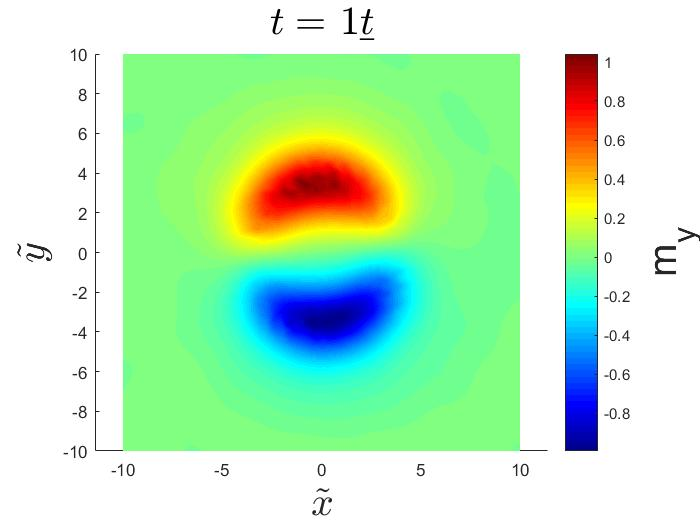
\includegraphics[width=\linewidth]{Figures/StaticSkyrmionMyT1.jpg}
  \caption{}
  \label{fig:StaticSkyrmionMyT1}
\end{subfigure}
\begin{subfigure}{.3\textwidth}
  \centering
  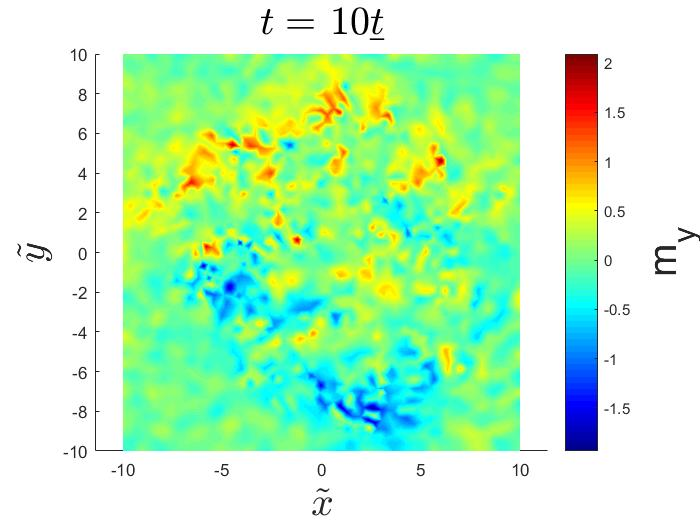
\includegraphics[width=\linewidth]{Figures/StaticSkyrmionMyT10.jpg}
  \caption{}
  \label{fig:StaticSkyrmionMyT10}
\end{subfigure}

\begin{subfigure}{.3\textwidth}
  \centering
  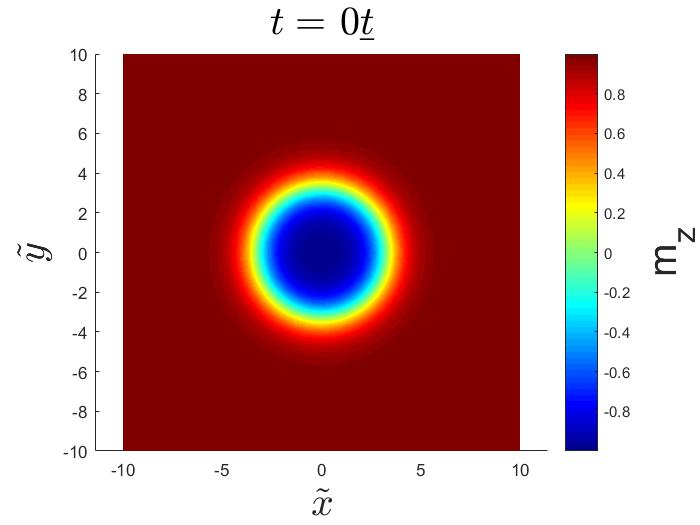
\includegraphics[width=\linewidth]{Figures/StaticSkyrmionMzT0.jpg}
  \caption{}
  \label{fig:StaticSkyrmionMzT0}
\end{subfigure}
\begin{subfigure}{.3\textwidth}
  \centering
  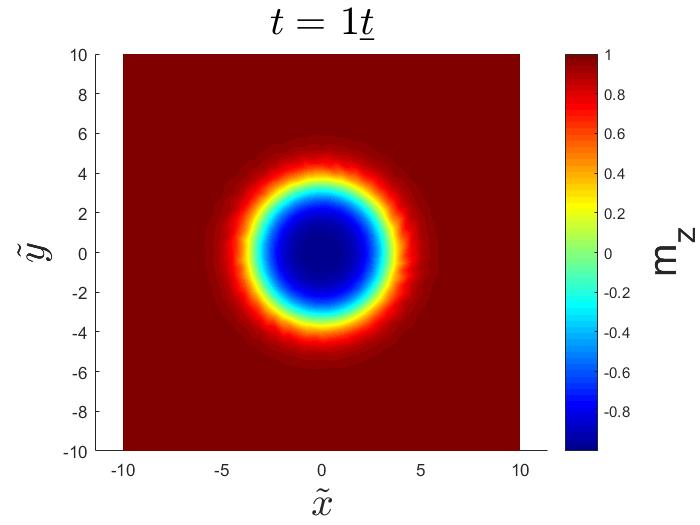
\includegraphics[width=\linewidth]{Figures/StaticSkyrmionMzT1.jpg}
  \caption{}
  \label{fig:StaticSkyrmionMzT1}
\end{subfigure}
\begin{subfigure}{.3\textwidth}
  \centering
  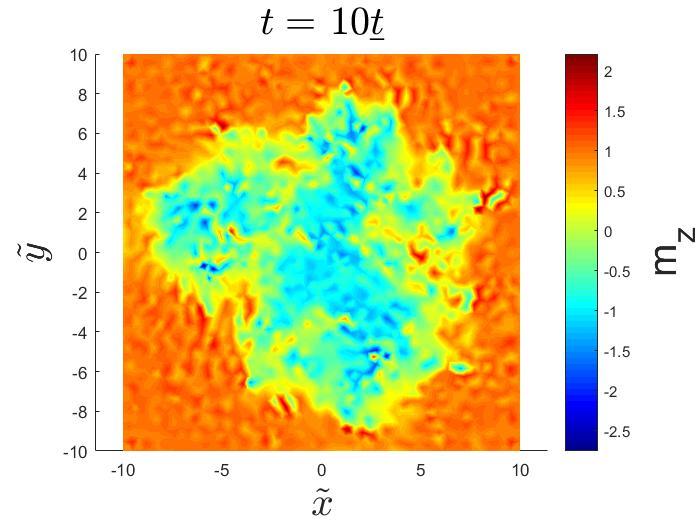
\includegraphics[width=\linewidth]{Figures/StaticSkyrmionMzT10.jpg}
  \caption{}
  \label{fig:StaticSkyrmionMzT10}
\end{subfigure}
\caption{Plots of the vector components $m_x$, $m_y$ and $m_z$ in the skyrmion plane for different times in the numerical simulation. The first row contains the data for $m_x$, the second for $m_y$ and the third for $m_z$. The first column shows the initial state, the second at a time $t=\underline{t}$ and the third at a time $t=10\underline{t}$.}
\label{fig:StaticSkyrmion}
\end{figure}
The results are shown in Figure \ref{fig:StaticSkyrmion}. At a time $t=\underline{t}$ there is not much change in the solution, but there is a slight counterclockwise rotation of the $m_x$ and $m_y$ values. After a time $t=10\underline{t}$, however, the solution has smeared out significantly from the initial state. More importantly, the values of the vector components exceed the allowed interval $\left[-1,1\right]$ by far, thereby breaking the normalization $m_x^2+m_y^2+m_z^2=1$ of the system. The LLG equation explicitly conserves the magnitude of the magnetization, so this is of particular interest when considering the stability of the code. Although we have three equations that we solve numerically, they are not independent of each other, as we can find the third vector component up to a sign once we have the solution of two. The numerical simulation does not seem to handle this well enough after a certain time, however. It is therefore a clear indication that the implemented solution method is not stable enough. There are several things that could cause this. If the boundary conditions are chosen incorrectly, this could affect the system. For this simulation Dirichlet boundary conditions corresponding to the numerical skyrmion solution at each point were chosen, and should therefore not affect the solution under the assumption that there is no dynamics. Another possible source of the instability is how the initial conditions are handled. The out of plane angle $\theta$ in the skyrmion profile has to be determined numerically from \eqref{eq:ODEtheta}. This is a differential equation with a singular point at $\tilde{r} = 0$, and we therefore settle by solving the equation down to a value close to zero. The solution of $\theta$ will also be needed arbitrarily close to zero, or at zero itself, when considering the entire skyrmion. A quick fix to this problem is shifting the $\tilde{r}$-values of the numerical solution of $\theta$ so that the $\theta$ values start at $\tilde{r}=0$ instead of $\tilde{r}=\epsilon$ (with $\epsilon$ here being set to $10^{-4}$). This is not a particularly good solution to the problem, as it introduces a small off-set to the solution of $\theta$ that will make the skyrmion profile not perfectly aligned with the effective field. However, as this off-set is so small, it is expected that any dynamics this will induce in the LLG equation will primarily go towards stabilizing the skyrmion to its proper stable form. What is more important about this fix is that it makes the function $\theta(\tilde{r})$ well defined at all points, so that $\mathbold{m} = \left(\sin\theta\cos\Phi,\sin\theta\sin\Phi,\cos\theta\right)$ is defined at all points in the skyrmion plane. To check if this fix is sufficient, we study the first and second derivatives of the magnetization, which appear in the effective field. The results are shown in Figure \ref{fig:SkyrmionDerivatives}.
\begin{figure}[h!]
\centering
\begin{subfigure}{.45\textwidth}
  \centering
  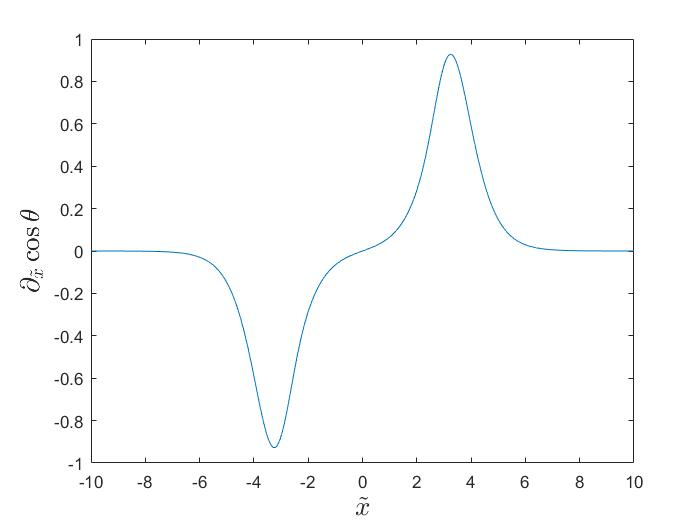
\includegraphics[width=\linewidth]{Figures/dCosTheta.jpg}
  \caption{}
\end{subfigure}
\begin{subfigure}{.45\textwidth}
  \centering
  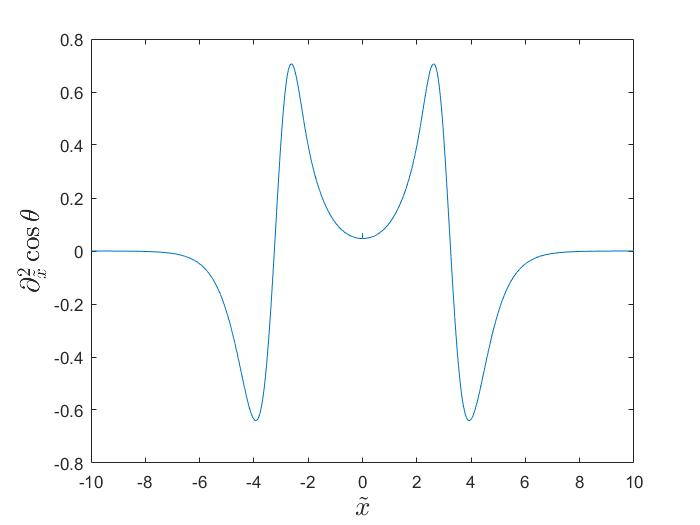
\includegraphics[width=\linewidth]{Figures/d2CosTheta.jpg}
  \caption{}
\end{subfigure}

\begin{subfigure}{.45\textwidth}
  \centering
  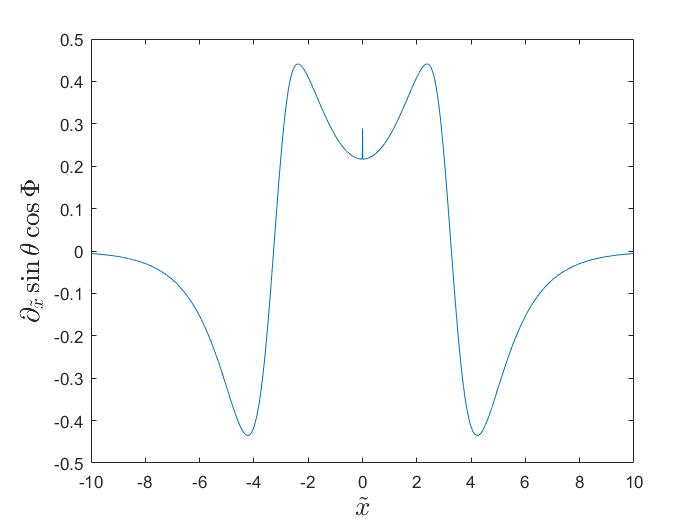
\includegraphics[width=\linewidth]{Figures/dSinThetaCosPhi.jpg}
  \caption{}
\end{subfigure}
\begin{subfigure}{.45\textwidth}
  \centering
  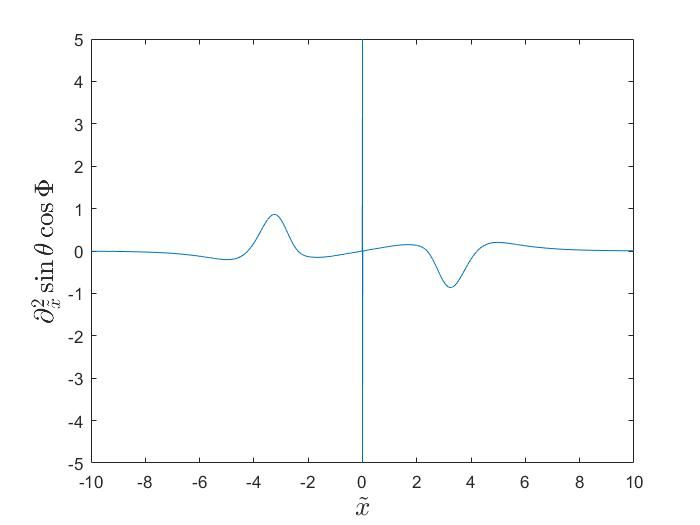
\includegraphics[width=\linewidth]{Figures/d2SinThetaCosPhi.jpg}
  \caption{}
\end{subfigure}
\caption{First and second derivatives of $m_x$ and $m_z$ in the $x$-direction. Every derivative has a discontinuity at $\tilde{x}=0$ except for the first derivative of $m_z$. The second derivative of $m_x$ has a singularity at $\tilde{x}=0$.}
\label{fig:SkyrmionDerivatives}
\end{figure}
As one can see, we still have an issue with discontinuities in the derivatives. For the $m_x = \sin\theta\cos\Phi$ case this could possibly stem from the $\cos\Phi$ factor, as $\Phi$ is not properly defined at $\tilde{r}=0$. As the first derivative of $m_x$ has a discontinuity while the first derivative of $m_z$ does not, and $m_z$ is independent of $\Phi$, it would back up this hypothesis. However, as $\sin\theta(\tilde{r}=0)=0$ a value for $\Phi$ at this point should not be necessary. But we also see that our fix of the $\theta$ solution cannot be without problems, as we also have a discontinuity in the second derivative of $m_z$, and this must stem from how we handle $\theta$. These discontinuities could therefore be an explanation for the instability in our numerical simulations. A last possible explanation for the instability is that while the LLG equation should conserve the magnitude of $\mathbold{m}$ by default due to the form of the equation, there is no explicit constriction in the solver that requires that $m_x^2+m_y^2+m_z^2=1$. As the numerical solutions are based on approximations, if there is a small perturbation that makes $m_x^2+m_y^2+m_z^2\neq1$ the solver will not necessarily attempt to adjust the magnitude of $\mathbold{m}$ back to unity, and this perturbation can then increase until the components of $\mathbold{m}$ reach unrealistic values. From this point on the results of the simulation are of absolutely no interest, as the input to the next time step is outright wrong.

\subsection{Spin-transfer torque driven dynamics}
In the previous subsection we saw that the numerical simulation proved to be unstable even in a case that should involve no dynamics. However, up to the time $t=\underline{t}$ it was more or less stable, with some deformations of the initial state that should not be present. Despite the fact that the results yielded by the simulations cannot be relied entirely upon, even up to this time, we will attempt to introduce some dynamical terms in the LLG equation and solve this to a time $t=\underline{t}$ and compare this with our analytical results. While the quantitative behavior may be too inaccurate for us to judge if the numerical results agree with our analytical ones, hopefully we can still see if the qualitative behavior is the same. 
\begin{figure}[h!]
\centering
\begin{subfigure}{.45\textwidth}
  \centering
  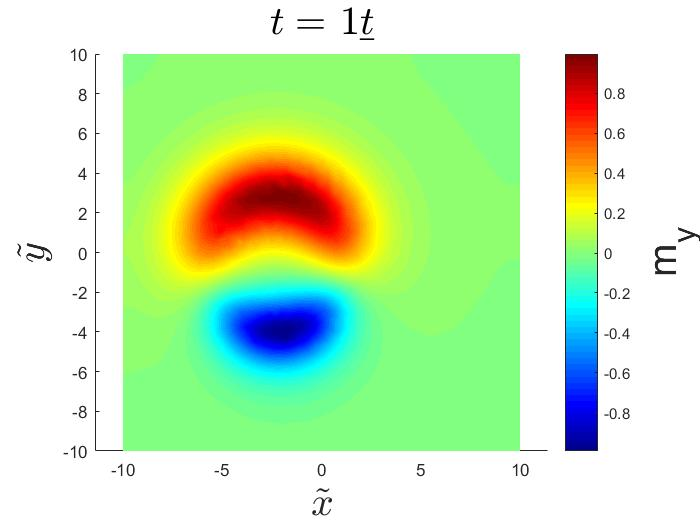
\includegraphics[width=\linewidth]{Figures/SkyrmionMySTTa1b3.jpg}
  \caption{}
\end{subfigure}
\begin{subfigure}{.45\textwidth}
  \centering
  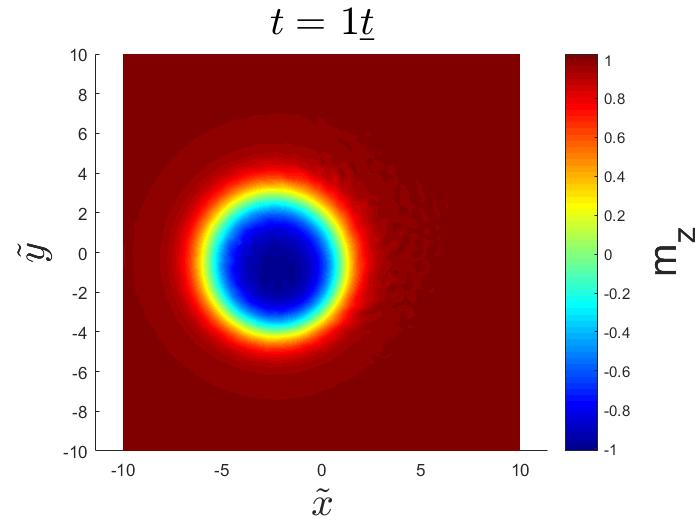
\includegraphics[width=\linewidth]{Figures/SkyrmionMzSTTa1b3.jpg}
  \caption{}
\end{subfigure}
\caption{Plots of $m_y$ and $m_z$ at a time $t=\underline{t}$ for a skyrmion driven by spin transfer torques. The skyrmion considered has $C=0.5551$ and the applied current gives a characteristic velocity $b_J\approx 178$ m/s ($b_J=1$ in dimensionless units). The values of the damping parameters were set to $\alpha=1.0$ and $\beta=3.0$. The geometric center of the skyrmion is found to be approximately $\left(-2.20, -0.85\right)$ from the plot of $m_z$.}
\label{fig:SkyrmionMotionSTTa1b3}
\end{figure}
The first test we do is on a skyrmion with $A=\SI{10}{pJ/m}$, $K=0.17$ MJ/m$^3$, $D=1.75$ mJ/m$^2$, $M_s=0.96$ MA/m. The characteristic velocity $b_J$ due to the spin transfer torque from the current is set to be unity in dimensionless units. Lastly we choose large damping parameter values ($\alpha=1.0$ and $\beta=3.0$) to make the impact of the different types of STT clear. The results are shown in Figure \ref{fig:SkyrmionMotionSTTa1b3}. While there is a clear deformation of the $m_y$ component, the $m_z$ component has more or less undergone a rigid motion, and all the magnetization components have reasonable values in the range $\left[-1,1\right]$. By looking closely at the plot of $m_z$ one can find that the location of the skyrmion core is approximately $\left(-2.20, -0.85\right)$. Using our analytical model in \eqref{eq:ElectricalSkyrmionVComponents} we would expect the core to be at $\left(-2.47, -0.88\right)$. The numerical result is then rather close to what we would expect from our analytical model. The discrepancy can perhaps be due to the deformation of the $m_y$ component, as our analytical model was made under the assumption of a rigid motion of the skyrmion. Whether the deformation is something that would actually occur in the physical case is not something we can say with accuracy, as we have already determined in the last subsection that the simulations give some deformations in cases where there should be none. In any case, the result we get agrees very well qualitatively with our analytical ones. We have a main velocity component along the direction of the conduction electrons, and also a component perpendicular to the current direction due to the skyrmion Hall effect as $\alpha\neq\beta$. When $\alpha=\beta$, however, we expect this perpendicular component from the skyrmion Hall effect to vanish. To check this we run a simulation with similar parameters as before, except now we set $\alpha=\beta=1$. The analytical model would now expect the skyrmion to have a velocity $\mathbold{v}=-b_J\mathbold{\hat{x}}$. The $m_z$ component resulting from this simulation is presented in Figure \ref{fig:SkyrmionMotionSTTa1b1}, and its center is at $\left(-1,0\right)$, in complete agreement with our analytical model. In addition, we do not have any deformations of significant magnitude in any of the magnetization components.
\begin{figure}[h!]
\centering
  \centering
  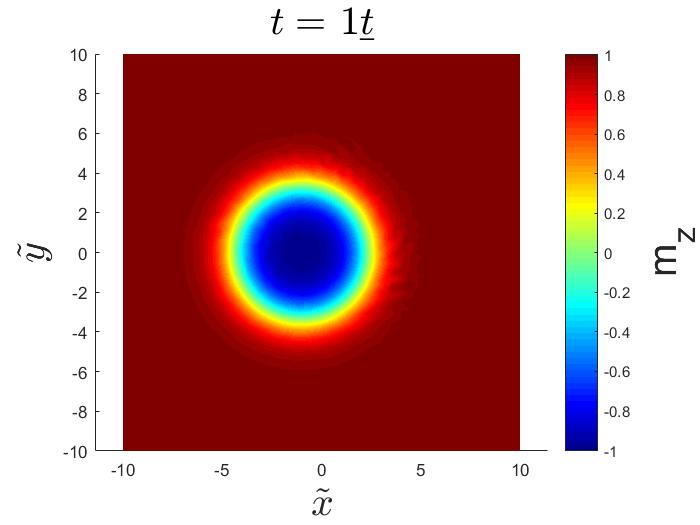
\includegraphics[width=.6\linewidth]{Figures/SkyrmionMzSTTa1b1.jpg}
\caption{Plot $m_z$ at a time $t=\underline{t}$ for a skyrmion driven by spin transfer torques. The skyrmion considered has $C=0.5551$ and the applied current gives a characteristic velocity $b_J\approx 178$ m/s ($b_J=1$ in dimensionless units). The values of the damping parameters were set to $\alpha=\beta=1.0$. The geometric center of the skyrmion is found to be $\left(-1, 0\right)$ from the plot of $m_z$.}
\label{fig:SkyrmionMotionSTTa1b1}
\end{figure}

\subsection{The effects of RSOC on the current driven dynamics}
We now move on to check the effects of RSOC on the dynamics of the skyrmion. It turns out that there is no time in the simulation that is large enough to see these effects that does not break the normalization of the magnetization to a significant degree. These values outside of the range $\left[-1,1\right]$ are local, however, so we still attempt an analysis. Before we start the analysis it should be noted that the results shown and discussed in this section should be taken with a grain of salt, as the code shows clear signs of instability. As this instability also appears at $t=\underline{t}$, and does not increase significantly at $t=2\underline{t}$, we run our simulation up to $t=2\underline{t}$ in this subsection. The dynamical effects of RSOC only appears when we have an applied current in the material. To see its effects it is therefore best to compare the current driven dynamics of a skyrmion in a material with and without RSOC. The strength of DMI is set to be the same in both systems, despite the fact that the presence of RSOC will influence this. For this simulation we use the data for the cobalt nanotracks in Table \ref{tab:PhysicalConstants}, and apply a current in the $x$-direction corresponding to $b_J = 1$ in its dimensionless value. We let the damping constants take on large values $\alpha=\beta=1$ for it to be easier to recognize the effects of RSOC, as it is expected that the RSOC correction is proportional to $\beta$. The simulation results are shown in Figure \ref{fig:SkyrmionRSOC}. The first thing we notice is that there is significant more deformation in the system with RSOC than the one without. This could again be due to the instability of the code, having RSOC present in the LLG equation makes the equations harder to solve. However, RSOC appears as fields in the LLG equation, and for large currents these fields can reach an order of magnitude comparable to the effective field. It is therefore not that unexpected that RSOC causes a deformation of the skyrmion, as the skyrmion magnetization profile is no longer perfectly aligned with the experienced magnetic field. The second thing one notices is that the location of the skyrmion core is not the same in the material with RSOC and the one without. The presence of RSOC shifts the core in the positive $x$- and $y$-direction. This is behavior that is similar to what is predicted by \eqref{eq:ElectricalSkyrmionVComponents} (remember that $R$ is negative for positive $\alpha_R$ and $b_J$). Analytically the core should be located at $\left(-1.17, 0.29\right)$ in the presence of RSOC, while numerically the core is approximately found to be located at $\left(-0.90, 0.35\right)$. The results are not that different, and can possibly be due to the deformation of the skyrmion or the instability of the code. What is most important to note is that the qualitative effects of RSOC on the current driven skyrmion dynamics agree rather well with one another.
\begin{figure}[h!]
\centering
\begin{subfigure}{.45\textwidth}
  \centering
  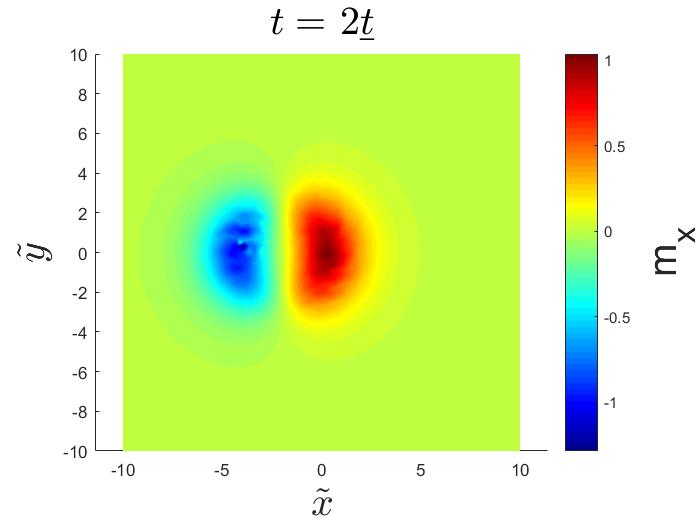
\includegraphics[width=\linewidth]{Figures/SkyrmionMxRSOCR0.jpg}
  \caption{}
\end{subfigure}
\begin{subfigure}{.45\textwidth}
  \centering
  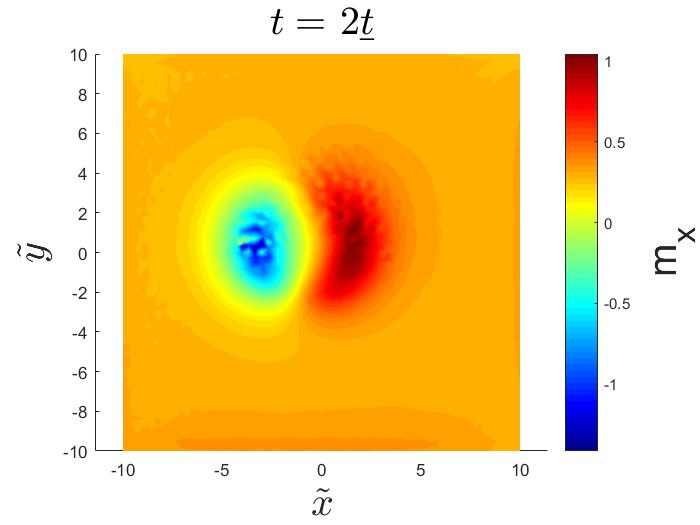
\includegraphics[width=\linewidth]{Figures/SkyrmionMxRSOC.jpg}
  \caption{}
\end{subfigure}

\begin{subfigure}{.45\textwidth}
  \centering
  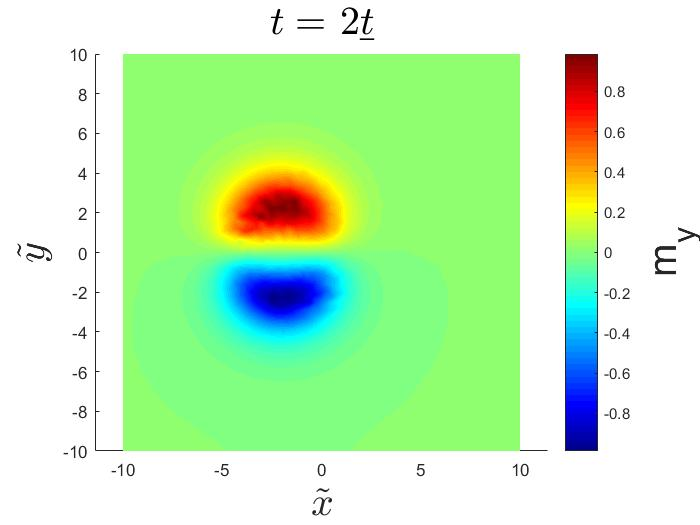
\includegraphics[width=\linewidth]{Figures/SkyrmionMyRSOCR0.jpg}
  \caption{}
\end{subfigure}
\begin{subfigure}{.45\textwidth}
  \centering
  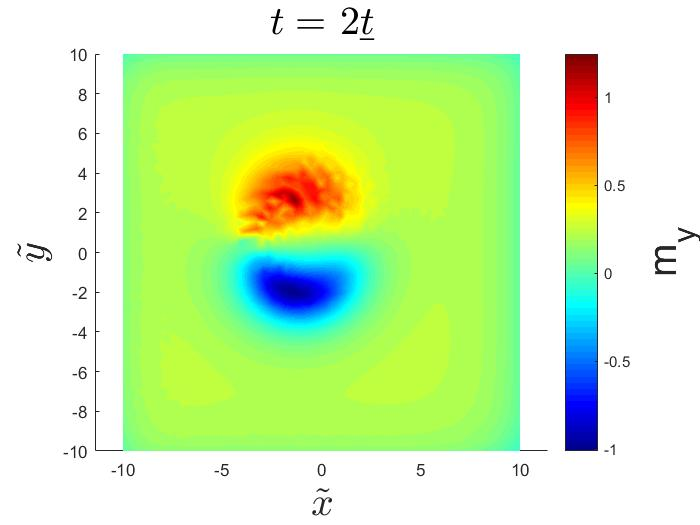
\includegraphics[width=\linewidth]{Figures/SkyrmionMyRSOC.jpg}
  \caption{}
\end{subfigure}

\begin{subfigure}{.45\textwidth}
  \centering
  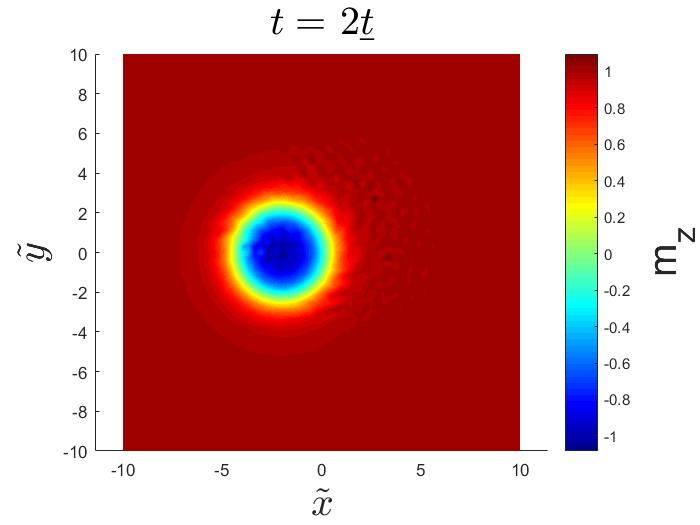
\includegraphics[width=\linewidth]{Figures/SkyrmionMzRSOCR0.jpg}
  \caption{}
\end{subfigure}
\begin{subfigure}{.45\textwidth}
  \centering
  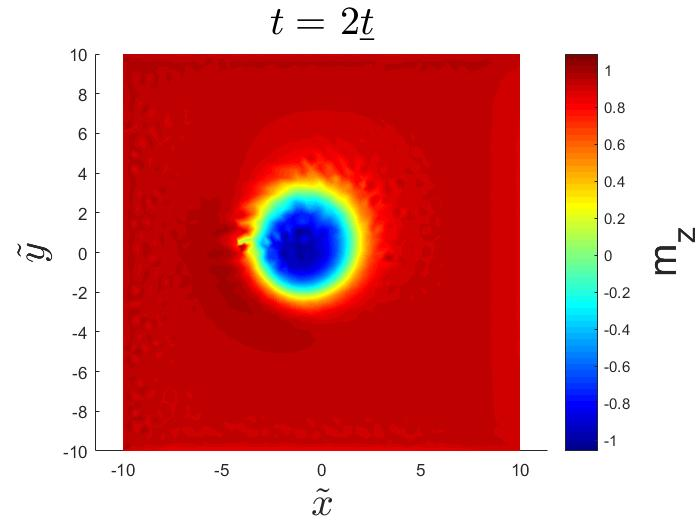
\includegraphics[width=\linewidth]{Figures/SkyrmionMzRSOC.jpg}
  \caption{}
\end{subfigure}
\caption{$\alpha_R=5.1$ peV$\cdot$m, $b_J=1$, $C=0.75$, $\alpha=\beta=1$. The skyrmion core is located at $\left(-2,0\right)$ without RSOC, and at approximately $\left(-0.90,0.35\right)$ with RSOC. }
\label{fig:SkyrmionRSOC}
\end{figure}

\subsection{Electric field driven dynamics}
The last effect to check numerically is then the dynamics induced by an inhomogeneous electric field applied perpendicular to the skyrmion plane. The problem with simulating these effects is that for reasonably scaled electric field gradients, such that the overall change in the free energy in the vicinity of the skyrmion is rather small, the time scale needed to see the effects is quite large compared to $\underline{t}$. At these time scales we have seen that the simulations become unstable, and this instability renders any output we may get useless. To get a motion of the skyrmion that we can see at a time scale $\underline{t}$ we can, however, use a very steep electric field gradient. The ones used in these simulations were set so that $\eta E_{x/y}\underline{r} = 0.2 K$. This method is not entirely unproblematic either, not even considering that this is a much stronger modification of the anisotropic energy than we can accomplish with an electric field. With a gradient this steep there is a considerable change in the free energy. If we consider the example with $\eta E_{x}\underline{r} = 0.2 K$ the total anisotropic energy at $\tilde{x}=-5$ is zero, while at $\tilde{x}=5$ is twice that of the original anisotropic energy without an applied electric field. This should cause noticeable deformations in the skyrmion, as the change in the effective field becomes so great that the magnetization of the skyrmion is not even close to being the stable solution. For small time scales these deformations will hopefully not be that dominant, however. There are two effects we would like to check for the electric field driven motion of the skyrmion; in the undamped limit the skyrmion should move perpendicular to the electric field gradient, while in the presence of damping there should also be a velocity component in the opposite direction of the gradient. We therefore run simulations for two different values of $\alpha$ for each gradient direction. We choose a value $\alpha=0.01$ that should show primarily the motion in the undamped case, and a value $\alpha=0.7$ to introduce the velocity component due to damping. The value of $\alpha=0.7$ is chosen to get the maximum velocity component in the opposite direction of the field gradient. This happens when $\alpha_C=1$, which would correspond to $\alpha=0.7$ for a skyrmion with $C=0.75$, as we get when using the values for the cobalt nanotracks in Table \ref{tab:PhysicalConstants}. The simulation results for the $m_z$ component at a time $t=2\underline{t}$ are shown in Figure \ref{fig:SkyrmionEField}. As we can see there is some deformation of the skyrmion, primarily an elongation along the axis where we apply an electric field gradient. If one studies the plots closer, one can also see that the position of the core has moved slightly, although this is hard to see directly from the plots as presented here.

We will now compare the analytical and numerical core positions using \eqref{eq:ElectricalSkyrmionVComponents} and Figure \ref{fig:SkyrmionEField}. The analytical core locations are given by $\left(-0.01, -0.86\right)$ and $\left(-0.43, -0.43\right)$ for a gradient in the $x$-direction and a damping parameter $\alpha=0.01$ and $\alpha=0.7$ respectively. For a gradient in the $y$-direction the locations are $\left(0.86,-0.01\right)$ and $\left(0.43, -0.43\right)$ for $\alpha=0.01$ and $\alpha=0.7$ respectively. The analytical results are in good agreement with the velocity component perpendicular to the gradient found numerically, but there is some discrepancy in the velocity component in the opposite direction of the gradient that is proportional to $\alpha$. Qualitatively the damped velocity component behaves correctly, but quantitatively it is a bit off comparing to the perpendicular velocity component. This could possibly stem from the elongation of the skyrmion along the gradient axis, as the core is chosen to be where the $m_z$ component is minimal, but this is no longer the geometric center of the skyrmion. 
\begin{figure}[h!]
\centering
\begin{subfigure}{.45\textwidth}
  \centering
  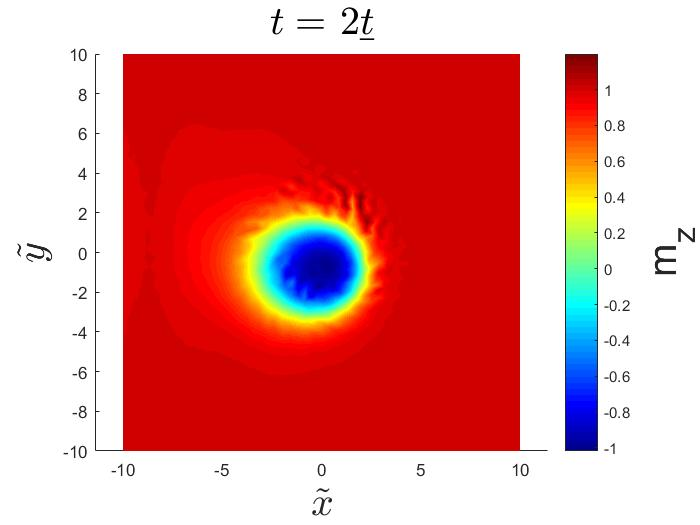
\includegraphics[width=\linewidth]{Figures/SkyrmionExA001.jpg}
  \caption{}
\end{subfigure}
\begin{subfigure}{.45\textwidth}
  \centering
  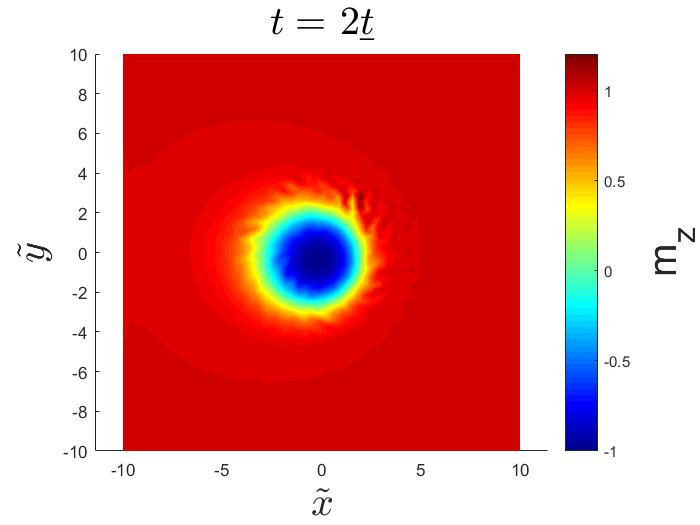
\includegraphics[width=\linewidth]{Figures/SkyrmionExA07.jpg}
  \caption{}
\end{subfigure}

\begin{subfigure}{.45\textwidth}
  \centering
  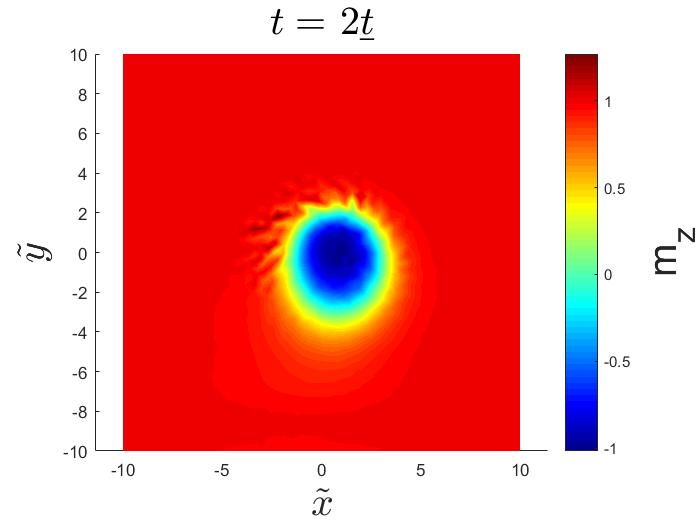
\includegraphics[width=\linewidth]{Figures/SkyrmionEyA001.jpg}
  \caption{}
\end{subfigure}
\begin{subfigure}{.45\textwidth}
  \centering
  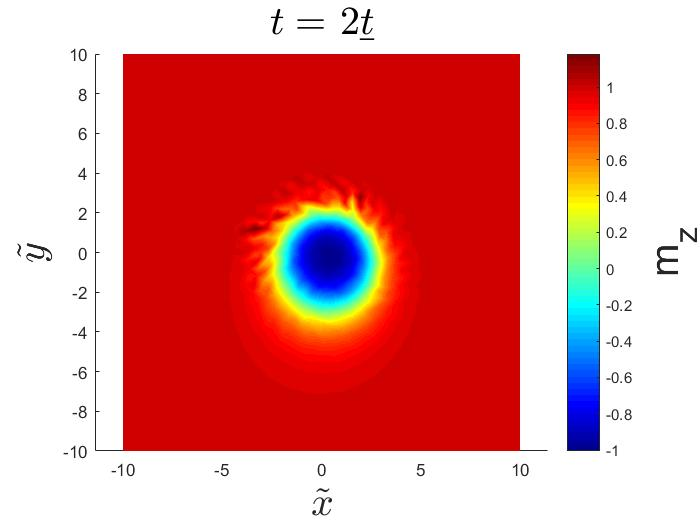
\includegraphics[width=\linewidth]{Figures/SkyrmionEyA07.jpg}
  \caption{}
\end{subfigure}
\caption{The $m_z$ component of a skyrmion with $C=0.75$ at a time $t=2\underline{t}$ after applying an electric field gradient to the system at $t=0$. In \textbf{(a)} and \textbf{(b)} we have applied a gradient $E_x$ in the $x$-direction, while in \textbf{(c)} and \textbf{(d)} we have applied a gradient $E_y$ in the $y$-direction. The electric field is given by $E = (E_x x+E_yy)\mathbold{\hat{z}}$, and the field strength is given by $\eta E_{x/y}\underline{r} = 0.2 K$, where we have used the materialistic properties of cobalt nanotracks. In \textbf{(a)} and \textbf{(c)} the damping parameter is $\alpha = 0.01$, while in \textbf{(b)} and \textbf{(d)} it is $\alpha=0.7$. The core locations are found to be approximately \textbf{(a)} $\left(0,-0.75 \right)$, \textbf{(b)} $\left(-0.2,-0.4 \right)$, \textbf{(c)} $\left(0.75,0 \right)$, \textbf{(d)} $\left(0.4,-0.2 \right)$.}
\label{fig:SkyrmionEField}
\end{figure}

As a final comment on the electric field control of the skyrmion motion we would like to discuss what is a realistic size of the electric field gradient, and how this may be utilized in skyrmion motion. By rewriting \eqref{eq:ElectricalSkyrmionVComponents}, we can express the electric field gradients as
\begin{subequations}
\begin{align}
    E_x &= -\frac{1}{C_E}\left[\left(\beta+R\right)b_J + \alpha\dot{x}_0+\dot{y}_0\right], \\
    E_y &= \frac{1}{C_E}\left[b_J+\dot{x}_0-\alpha\dot{y}_0\right].
\end{align}
\end{subequations}
One use of the electric field control of the skyrmion motion is to cancel out the perpendicular velocity component when the skyrmion is dynamically driven by a spin-polarized current. We can then estimate the size of the gradient necessary to accomplish this based on the expression above. For simplicity we assume an undamped case with $\alpha=\beta=0$, so that the $\dot{y}_0$ component can be cancelled out by an electric field gradient in the $y$-direction. The magnitude of this gradient then becomes
\begin{align}
    \eta E_y\underline{r} = \frac{2\mu_0M_s\underline{r}}{\gamma' I_3}\left(\dot{x}_0+b_J\right).
\end{align}
For a current density $j_e = 10^{10}$ A/m$^2$ the size of $b_J$ is approximately $\SI{1}{m/s}$. Typically $\dot{x}_0$ will be of the same magnitude as $b_J$, so we will assume this also to be $\SI{1}{m/s}$. In the cobalt nanotrack case, we would then require an electric field gradient of the magnitude $\eta E_y\underline{r}/K = 10^{-3}$ to cancel out the perpendicular velocity component, while for the Ir|Co|Pt multilayer system we would require $\eta E_y\underline{r}/K = 3\cdot10^{-3}$. This is a much more feasible field gradient than the one used in the numerics to illustrate the dynamics (which was $\eta E_y\underline{r}/K = 0.2$), as it does not require a very considerable change in the perpendicular magnetic anisotropy. In addition, as the free energy is slowly varying in the vicinity of the skyrmion, it is unlikely to cause any deformations of significance. 